\BourbakiUnnumberedChapter{历史注记}{历史注记（第四、五章）}

（第四章和第五章）

（方括号中的数字指本注记末尾的参考文献。）

交换域的理论——以及与之密切相关的多项式理论——直接源于直到19世纪中叶仍构成经典代数学主要对象的内容：代数方程的求解，以及与之等价的几何作图问题。

一旦人们试图求解一个次数为 \(>1\) 的代数方程，就会发现自己面临着全新的计算困难，因为不再可能通过对数据进行“有理”运算来确定未知量。这一困难必定在很早的阶段就被察觉到了；巴比伦人最重要的贡献之一，应当是他们能够将二次和四次方程的求解归结为一种新的代数运算，即开平方（正如流传下来的文本中许多以这种方式求解的数值方程所表明的那样（{[}1{]}，第183—193页））。就形式计算而言，古代在代数方程求解问题上从未超越这一点；古典时期的希腊人实际上仅限于用几何语言重述巴比伦公式，而它们以代数形式的使用在希罗（公元100年）和丢番图之前没有文献记载。

希腊人是在一个相当不同的方向上取得了决定性的进展。关于巴比伦人如何构想和计算非完全平方整数的平方根，我们所知甚少*；在流传下来的关于这一问题的罕见文本中，他们似乎满足于相当粗略的近似方法（{[}1{]}，第33—38页）。毕达哥拉斯学派曾以相当严格的方式确定了可公度量的概念，并赋予其近乎宗教的性质，却未能始终坚持这一观点；也许正是反复尝试有理地表示 \(\sqrt{2}\) 的失败，最终导致他们证明了该数是无理数**。

我们已在别处说过（参见第三卷第四章的历史注记），这一发现如何成为数学史上的分水岭，深刻地影响了希腊人对“数”的概念，并促使他们创造了一种纯粹几何特征的代数，以便为不可公度比找到一种表示方式（或者也许是一种“存在性”证明），因为他们拒绝将这些比视为数。在大多数情形，他们把一个代数问题归结为两条适当选取的辅助平面曲线的交点，或归结为相继若干次确定这样的交点。一些权威性甚低的晚期传统把这类作图的第一个分类的引入归功于柏拉图，这一分类注定有着漫长而辉煌的历程：似乎出于哲学而非数学的原因，所谓的“尺规作图”，即其中出现的仅有的辅助曲线为直线和圆的那些作图，被单独列为一类*。无论如何，欧几里得在他的《几何原本》 {[}2{]} 中仅限于专门处理可以这种方式解决的问题（尽管没有用特定名称来刻画它们）；这一情况无疑极大地促使后世数学家将注意力集中在这些问题上。但我们今天知道**，可以用“尺规”求解的代数方程是一种非常特殊的类型；特别地，一个不可约方程

立即给出 \(\sqrt{5}\) 的无理性的一个证明，而且他提出了一个假设（遗憾的是没有任何文本支持这一假设），即毕达哥拉斯学派正是以这种方式发现了无理数（K. von FRITZ，Ann. of. Math.，第46卷（1945年），第242页）。

* 关于这一原则，人们还将平面曲线分类为“平面轨迹”（直线和圆）、“立体轨迹”（圆锥曲线，通过平面截取立体——圆锥得到）的作法归功于柏拉图，所有其他曲线则统称为“τόποι γραμμικοι”。值得注意的是，这一分类的影响甚至延伸到了笛卡尔，他在其《几何学》中将次数为2n−1和2n的方程归入同一“属”，无疑是因为次数为1或2的方程通过“平面轨迹”的交点求解，而次数为3或4的方程通过“立体轨迹”的交点求解。

** 确定一条直线与一个圆（或两个圆）的交点，等价于求一个二次方程的解，该方程的系数是所考虑的直线和圆（或两个圆）的方程系数的有理函数。由此容易推出，从给定点“用尺规”作出的点的坐标属于有理数域Q的一个扩域L，其构造如下：若K是通过将给定点的坐标添加到Q而得到的域，则存在一个递增序列 \((\mathrm{L}_{i})_{0\leq i\leq n}\) ，其中的域都介于K和L之间，满足条件 \(K=L_{0}\) 、\(L=L_{n}\) 、\([L_{i}:L_{i-1}]=2\) （\(1\leq i\leq n\) ）。通过对n进行归纳，我们推出由L生成的伽罗瓦扩域N在K上的次数是2的幂；反之可以证明，若此条件成立，则存在一个序列 \((\mathrm{L}_{i})\) ，其中各域介于K和L之间且具有上述性质，因此所提出的问题可以用尺规求解（参见N. TSCHEBOTARÖW，Grundzüge der Galoisschen Theorie（H. Schwerdtfeger译），格罗宁根（P. Noordhoff出版社），1950年，第351页）。

三次（在有理数域上）的方程不能用这种方式求解，而希腊人很早就遇到了一些至今仍很著名的三次问题，例如倍立方（求解 \(x^3 = 2\) ）以及角的三等分；另一方面，化圆为方问题使他们面对一个超越性问题。我们发现，为了解决这些问题，他们引入了许多曲线，既有代数曲线（圆锥曲线、狄奥克勒斯的蔓叶线、尼科梅德斯的蚌线），也有超越曲线（狄诺斯特拉托斯的割圆曲线、阿基米德螺线）；所有这些不可避免地促使他们对这些不同的曲线进行独立研究，从而为解析几何、代数几何以及无穷小演算的未来发展铺平了道路。但这些方法对代数方程的求解没有带来任何进展*，而古代唯一对这一问题作出显著贡献并对中世纪和文艺复兴时期的代数学家产生持久影响的著作，是欧几里得《几何原本》 {[}2{]} 的第十卷；在这本书中（其中主要成果被某些历史学家归于泰阿泰德），他考察了由多个根式组合得到的表达式，例如 \(\sqrt{\sqrt{a} \pm \sqrt{b}}\) （\(a\) 和 \(b\) 为有理数），给出了这些表达式为无理数的条件，将它们分成众多的类别（并证明这些类别互不相同），并研究了这些不同的无理数之间的代数关系，例如我们今天会写成

\[
\sqrt {\sqrt {p} + \sqrt {q}} = \sqrt {\frac {1}{2} (\sqrt {p} + \sqrt {p - q})} + \sqrt {\frac {1}{2} (\sqrt {p} - \sqrt {p - q})};
\]

所有这些都用《几何原本》中惯用的几何语言表述，这使得论述显得尤为繁密而艰涩。

古典希腊数学衰落之后，与代数方程相关的概念经历了演变。毫无疑问，在整个古典时期，希腊人掌握了平方根无限逼近的方法，但遗憾的是，我们对这些方法知之甚少**。

在印度人那里，后来又在阿拉伯人及其中世纪的西方效仿者那里，各阶开方成为一种运算，它倾向于被看成与代数的有理运算具有同等地位的基本运算，并且像后者一样，用越来越便于在计算中处理的符号来表示*。二次方程的理论在中世纪得到了完善（根的个数、负根、不可能情形、重根），四次方程的理论也是如此，它们为“用根式”求解方程提供了公式的范例，几个世纪中代数学家们都试图仿照这些范例，为更高次方程的求解建立类似的公式，首先便是三次方程。比萨的莱昂纳多在13世纪主要负责将阿拉伯科学引入西方，他认识到，无论如何，欧几里得在第十卷中分类的无理数不能用于此目的（在一个充满这类证明的理论中，这又是一个新的不可能性证明），并且我们看到他已经对立方根尝试了类似的计算，得到了诸如以下的关系：

\[
\sqrt [ 3 ]{1 6} + \sqrt [ 3 ]{5 4} = \sqrt [ 3 ]{2 5 0},
\]

类似于欧几里得关于平方根的公式（我们实际上在阿拉伯人那里能找到更早的例子）。但还要经过三个世纪徒劳无功的努力，直到16世纪初，希皮奥内·德尔·费罗才最终得到方程 \(x^3 + ax = b\) 的求解公式：

\[
x = \sqrt [ 3 ]{\frac {b}{2} + \sqrt {\left(\frac {b}{2}\right) ^ {2} + \left(\frac {a}{3}\right) ^ {3}}} + \sqrt [ 3 ]{\frac {b}{2} - \sqrt {\left(\frac {b}{2}\right) ^ {2} + \left(\frac {a}{3}\right) ^ {3}}}.\tag{1}
\]

我们在此不描述这一轰动性发现中引人入胜的一面——它引发的塔尔塔利亚一方与卡尔达诺及其学派之间的争执——也不描述作为主角的学者们那些往往饶有趣味的人物形象。但我们必须指出卡尔达诺及其弟子们在方程论中带来的决定性进展。卡尔达诺对使用负数的反感不如其同时代的大多数人强烈，他因此观察到三次方程可能有三个根，而四次方程有四个根（{[}3{]} ，第IV卷，第259页），并指出 \(x^3 + bx = ax^2 + c\) （他知道如何消去其中 \(x^2\) 项的一个方程）的三个根之和总等于 \(a\) （同上）。无疑受这一关系及其一般特征的直觉引导，他最先有了根的重数这一概念的初步想法；尤其是，他大胆地（并非没有修辞上的谨慎）对含有负数平方根的表达式进行形式计算。他很可能是被下述事实引到这一步的：当 \(\left(\frac{b}{2}\right)^{2} + \left(\frac{a}{3}\right)^{3} < 0\) 时（所谓的“不可约情形”，卡尔达诺在其中认识到三个实根的存在），这类表达式在使用公式(1)时自然出现；无论如何，这一点由他的弟子R. 邦贝利清楚地表明，他在其《代数学》（{[}4{]} ，第293页）中证明了关系

\[
\sqrt [ 3 ]{2 + \sqrt {- 1 2 1}} = 2 + \sqrt {- 1}
\]

并且他注意以已经非常接近现代阐述的形式明确给出复数运算的规则*。最后在1545年，卡尔达诺的另一个学生L. 费拉里借助一个三次的辅助方程**成功地求解了一般的四次方程。

在如此迅速的进展之后，接下来的时期，直到18世纪中叶，几乎未曾发展意大利学派引入的新思想。得益于他在代数记号方面带来的根本性进步，韦达得以一般性地表达代数方程的系数与根之间的关系，至少当根全为正数时如此***（{[}5{]} ，第158页）。更大胆的A. Girard {[}6{]} 毫不犹豫地断言（当然没有证明）：次数为 \(n\) 的方程恰好有 \(n\) 个根，只要把那些“不可能的根”计入，每个根按其重数计算，并且这些根满足韦达给出的关系；他还第一次得到了根的等幂和的表达式，直至指数4。

但17世纪的精神转向了其他方向，代数只是间接地从解析几何和无穷小演算的新发现中获益。因此，笛卡尔获得

* 邦贝利（{[}4{]}，第169页和第190页）将复数视为四个基元素的具有正系数的“线性组合”：“piu”（+1）、“meno”（-1）、“piu de meno”（+i）和“meno de meno”（-i）；特别地，他提出一条公理，即“piu”与“piu de meno”不能相加，这是线性无关概念的首次出现。

** 方程被化简为形式 \(x^4 = ax^2 + bx + c\) ，我们确定一个数 \(z\) 使得方程的右边

\[
(x ^ {2} + z) ^ {2} = (a + 2 z) x ^ {2} + b x + (c + z ^ {2})
\]

是完全平方，这就给出了关于 \(z\) 的一个三次方程。

韦达是古人的热情仰慕者，他系统性地避免在论证中引入负数；尽管如此，他有时仍能用自己的语言表达系数与根之间的关系，即使某些根为负；例如，若方程 \(x^3 + b = ax\) 有两个正根 \(x_1, x_2\) （ \(a > 0, b > 0\) ），韦达表明 \(x_1^2 + x_2^2 + x_1x_2 = a\) 与 \(x_1x_2(x_1 + x_2) = b\) （{[}5{]} ，第106页）。

代数曲线的切线（参见《历史注记》第四卷，第一至三章，第46页）与他的弟子胡德所陈述的代数方程根的重数判别准则有关（{[}7{]}，第433页及第507-509页）。无疑，代数函数与超越函数之间的区分也应归功于笛卡尔的影响，这与他在《几何学》中所引入的“几何”曲线与“机械”曲线之间的区分相平行（参见《历史注记》第四卷，第一至三章，第46页及第61页）。无论如何，这一区分在J.格雷戈里那里已表述得十分清楚，他在1667年甚至试图证明圆扇形面积不可能是弦和半径的代数函数*。“超越”这一术语出自莱布尼茨，他对这些分类问题在整个学术生涯中始终兴趣不减，并且大约在1682年，他通过证明sin x不是x的代数函数，发现了格雷戈里所追求结果的一个简单证明（{[}8{]}，第五卷，第97-98页）**。莱布尼茨与他的朋友契恩豪斯一道，实际上是当时少数仍对代数方程“根式”求解问题感兴趣的数学家之一。在其学术生涯初期，我们发现他研究三次方程的“不可约情形”，并使自己相信（事实上，其证明并不充分）在这种情况下不可能从解的公式中消去虚量（{[}9{]}，第547-564页）。大约在同一时期，他还尝试用根式求解五次方程，但同样未获成功；后来当契恩豪斯声称通过形如y = P(x)的变换（其中P是适当选取的四次多项式）使方程除首尾两项外的所有项都消失，从而解决该问题时，莱布尼茨立刻注意到确定P(x)系数的方程次数为 \textgreater{} 5，并认为该方法注定失败（{[}9{]}，第402-403页）。

似乎是新分析的需求逐渐重新点燃了对代数的兴趣。有理分式的积分（由莱布尼茨和约翰·伯努利完成）以及与之密切相关的虚对数问题，为更深入地发展虚数运算提供了机会，并重新提起把多项式分解为一次因式的问题（“代数基本定理”）*。就在18世纪初，二项式方程 \(x^n - 1 = 0\) 的求解被科茨和棣莫弗化为将圆分成 \(n\) 等份的问题；因此，为了得到其根的“根式”表达式，只需知道当 \(n\) 为奇素数时如何做到这一点，而棣莫弗指出，代换 \(y = x + \frac{1}{x}\) 把问题归结为求解次数为 \((n - 1)/2\) 的一个方程的“根式”解。至于“基本定理”，在一般“根式”解的多次失败尝试（包括欧拉的几次尝试 {[}10{]} ）之后，人们开始倾向于先验的证明，而不使用解的显式公式。这里不深入讨论所提出方法的细节（这些方法后来在拉格朗日和高斯的证明中结出果实；参见第二卷第六、七章及第三卷第八章的历史注记），只需在此指出18世纪中叶人们看待这一问题的视角；人们承认（除了对一般性的模糊感觉之外没有任何别的理由，这种感觉无疑同A. 吉拉尔那里一样，来自系数与根之间存在关系的事实）次数为 \(n\) 的方程总有 \(n\) 个“理想的”根，对它们可以像对数那样进行运算，而无需知道它们是否是（实数或复）数；需要证明的是（必要时利用对理想根的运算），这些根中至少有一个是通常的复数**。在这种有缺陷的形式中，可以辨认出“形式添加”这一一般观念的最初萌芽，尽管有高斯的反对（{[}13{]} ，第III卷，第1页），它后来成为现代交换域理论的基础。

随着拉格朗日（{[}11{]} ， \(a\) ）与范德蒙德 {[}12{]} 的基本回忆录的发表，1770年开启了代数方程历史上一个新的决定性时期。此前一直独占统治地位的、多少带有偶然性的寻找求解公式的经验主义，被对所提问题以及能够解决它们的方法的系统分析所取代；这一分析在六十年后导致了伽罗瓦的最终成果。拉格朗日和范德蒙德都是从次数 \(\leqslant 4\) 的方程求解公式中根式的多重取值所引入的歧义出发的；这一事实早已引起欧拉（{[}10{]} ， \(a\) ）的注意，他除其他事情外还证明了，在德尔·费罗公式中应当如何把其中出现的根式关联起来，以便得到3个根而不是9个。拉格朗日指出，德尔·费罗公式中的每个立方根都可以写成形式 \(\frac{1}{3} (x_1 + \omega x_2 + \omega^2 x_3)\) ，其中 \(\omega\) 是一个单位立方根，而 \(x_1, x_2, x_3\) 是所给方程的根按某种顺序的排列，他还作出了一个基本的观察：三个根的函数 \((x_1 + \omega x_2 + \omega^2 x_3)^3\) 在这三个根的每一置换下只能取两个不同的值，这先验地解释了该方程的求解方法之所以成功。对四次方程求解方法的类似分析把他引导到四个根的函数 \(x_1 x_2 + x_3 x_4\) ，该函数在根的任意置换下仅取三个不同的值，因而是某个三次方程的根，其系数是给定方程系数的有理函数*；正如拉格朗日所说，这些事实构成了“解三次和四次方程的真正原理，也可以说是其形而上学**”（{[}11{]} ，a)，第357页）。在这些例子的引导下，他计划就一般情形研究：对于次数为 \(n\) 的方程，当根被任意置换时，根的有理函数 V 可能取到的值的个数 \(\nu\) ***（V 是这 \(n\) 个根的有理函数）；他由此实际上开创了（其术语仍紧密贴合方程论）群论和域论，并且已经运用与今天所用的相同原理得到了若干基本结果。例如，他证明了数 \(\nu\) 整除 \(n!\) ，所用的推理正是今天用来证明有限群的子群的阶整除该群的阶的那一推理。更值得注意的是他证明的定理：若 \(V_1\) 与 \(V_2\) 是根的两个有理函数，使得 \(V_1\) 与 \(V_2\) 在同样的诸置换下保持不变，则其中每一个都是另一个与方程系数的有理函数（这是伽罗瓦定理的一个特例，该定理把伽罗瓦扩张的子扩张刻画为其伽罗瓦群的不变量域）：“这个问题，”他说，“在我看来是方程论中最重要的问题之一，我们将给出的一般解将有助于为代数的这一部分带来新的光明。”（{[}11{]} ，a)，第374页）。

所有这些研究在拉格朗日看来自然只是预备性工作，为的是分析通过逐次化归为较低次的方程来求解代数方程的各种可能方法；正如他所证明的，这样的方法关系到构造根的有理函数，使其在根的置换下取少于 \(n\) 个值。无疑受到三次方程结果的引导，他就一般情形引入了“拉格朗日预解式” \(y_{k} = \sum_{h=1}^{n} \omega_{k}^{h} x_{h}\) ，其中 \(\omega_{k}\) 是 n 次单位根 \((1 \leqslant k \leqslant n)\) ，并清楚地表明这 n 个数的知识如何蕴含根 \(x_{k}\) 的知识，且一般地考察了 \(y_{k}\) 所满足的方程的次数；例如他证明，若 n 是素数，则诸 \(y_{k}^{n}\) 是一个 n-1 次方程的根，其系数是某个方程的一个根的有理函数，该方程的次数为 \((n-2)!\) ，而这些系数又可由所给方程的系数有理地表示。“这里，除非我弄错，”他总结道，“是方程求解的真正原理，也是最适于引导我们达到目的的分析；正如我们所见，一切都归结为一种组合演算，由此可以先验地求得应当期待的结果”（{[}11{]} ，a)，第403页）。

关于范德蒙德的回忆录，尽管独立于拉格朗日的著作，却在许多点上与后者有所接触，特别是在研究根的有理函数、使其在根的置换下取尽可能少的不同值这一思想*，以及他为此目的同样引入的“拉格朗日预解式”的研究上。他的工作远不具有拉格朗日工作的清晰性和一般性；然而在一点上他明显走得更远，即把同样的思想应用于分圆方程 \(x^n - 1 = 0\) ，其中 \(n\) 为奇素数。拉格朗日满足于指出这个方程可化为次数为 \(m = (n - 1)/2\) 的有理系数方程，而不试图在 \(n \geqslant 11\) 时求解它；范德蒙德则断言，后一方程的各拉格朗日预解式的 \(m\) 次幂是有理的，这是由 \(x^n - 1 = 0\) 的各个根之间的关系得出的；但他仅限于对 \(n = 11\) 验证这一断言的可靠性，而不作一般的论证。

直到30年后，范德蒙德宣布的结果才由C. F. 高斯**完全证明。他关于方程 \(x^n - 1 = 0\) （ \(n\) 为奇素数）的决定性成果，属于他那令人难忘的算术研究的总体计划（{[}13{]} ，第I卷，第413页及以下），它们尤其展示了他驾驭我们现今所称的循环群理论的娴熟技巧。在证明了多项式 \(\Phi_n(x) = (x^n - 1)/(x - 1)\) 对奇素数 \(n\) 不可约***之后，他想到把它的 \(n - 1\) 个根写成形式 \(\zeta^{g^{k}} = \zeta_{k} \quad (0 \leqslant k \leqslant n - 2)\) ，其中 \(g\) 是同余式 \(z^{n-1} \equiv 1 \pmod{n}\) 的一个本原根（用现代术语说，这相当于揭示出群 \(\Gamma\) ——方程 \(\Phi_{n}(x) = 0\) 的群——是循环群这一事实）。对每个除数 \(e\) （它整除 \(n - 1\) ），他关联起 \(f = (n - 1)/e\) 个“周期” \(\eta_{\nu} = \zeta_{\nu} + \zeta_{\nu + e} + \zeta_{\nu + 2e} + \cdots + \zeta_{\nu + (f - 1)e}\) （ \(1 \leqslant \nu \leqslant f\) ），并且他本质上证明了诸 \(\eta_{\nu}\) 的具有有理系数的线性组合构成一个域，它由 \(f\) 个周期 \(\eta_{\nu}\) 中的任何一个生成，且在有理数域上的次数为 \(f\) （这个域当然对应于 \(\Gamma\) 的阶为 \(e\) 的子群）。我们在此无法详述这一分析及其所蕴含的重要算术结论；只需指出，它特别使他得到了那个著名的定理，即边数等于形如 \(2^{2^{k}} + 1\) 的素数的正多边形可以用直尺和圆规作出*。至于方程 \(\Phi_{n}(x) = 0\) 的根式解，把周期理论应用于拉格朗日预解式的 \(f\) 次幂 \(\sum_{\nu=0}^{f-1} \omega^{\nu} \eta_{\nu}\) （其中 \(\omega^{f} = 1\) ）即可容易地得到**。

拉格朗日的同胞鲁菲尼的研究与《算术研究》同时代，直接承自拉格朗日；他们从拉格朗日停下的地方接着研究这一问题，目标在于证明“一般”***五次方程“用根式”求解的不可能性。鲁菲尼的证明冗长而晦涩，尽管多次修订，仍不完整；但它已经非常接近阿贝尔后来得到的（原则上正确的）证明。其主要意义在于引入了代换演算和群论的最初步概念，这

鲁菲尼发展了它们以表明，不存在方程5个根的一个函数，当根被任意置换时，它取多于2个且少于5个值。

我们已经在第一章的历史注记中说过，置换群理论的这第一个轮廓是如何在数年之后由柯西加以发展和系统化的。但是，尽管发展拉格朗日关于代换思想的必要概念由此逐渐明晰，仍然有必要以同样清晰的方式阐述域理论的基本原理。这正是鲁菲尼所缺乏的，而阿贝尔和伽罗瓦将在代数方程求解问题的最后阶段着手进行这项工作。

阿贝尔在其短暂的一生中始终未曾停止对这一问题的萦怀。几乎还在孩提时代，他就相信自己找到了一般五次方程根式求解的公式。后来，当他认识到自己的错误时，便不曾停歇，直到成功证明了这样的公式并不存在（{[}14{]} ，第I卷，第166页）。但他并未止步于此。当他的竞争者雅可比以分析学家的方式发展椭圆函数理论时，支配阿贝尔在这一问题上的工作的却是代数观点，其中心是椭圆函数分割方程的理论（{[}14{]} ，第I卷，第265、377页及多处）。他由此得到了一些新型的可根式求解的方程，其方法仿照高斯处理分圆方程的方法（{[}14{]} ，第I卷，第310和358页）*；从这一结果他上升到“阿贝尔”方程的概念，并在一篇著名的回忆录中证明了这类方程可根式求解（{[}14{]} ，第I卷，第478页）；正是在这个场合，他精确定义了给定域（由他所研究的方程的系数生成的域）上不可约多项式的概念**。最后，死神于1829年将他击倒，当时他正在攻克刻画所有可根式求解的方程这一一般问题，并且刚刚向克雷尔和勒让德通报了已非常接近伽罗瓦结果的研究（{[}14{]} ，第II卷，第219-243、269-270和279页）。

三年后，为这座大厦加冕的任务正是留给了他 \([15]\) 。与阿贝尔类似，但方式更为精确，他首先定义了（除名称外）一个量属于由给定量生成的域、添加的概念以及给定域上的不可约多项式。给定一个方程 \(F(x) = 0\) ，它没有重根，系数属于一个给定域 \(K\) ，他相继表明如何“总可以构造根的一个函数 \(V\) ，使得以一切可能的方式在该函数中置换根所得到的值没有一个等于另一个”，该函数“具有这样的性质：所给方程的所有根都可以表示为 \(V\) 的有理函数”，而且，若 \(V, V', V'', \ldots\) 是 \(V\) 所满足的不可约方程的根，则“若 \(a = f(V)\) 是所给方程的一个根，那么 \(f(V')\) 也是”（{[}15{]} ，第36-37页）；用现代术语说，他由此证明了 \(V\) ，同它在 \(K\) 上的任一共轭元一样，生成域 \(N\) （ \(F\) 的根的域）。然后他定义群 \(\Gamma\) （即 \(F\) 的群）为根 \(x_i\) 的通过代换 \(V\) 而得到的那些置换的集合：在把每个 \(x_i\) 表示成 \(V\) 的函数的有理表达式中，代入 \(V\) 的任何一个共轭元；他随即得到 \(K\) 的元素由在 \(\Gamma\) 的每一置换下不变这一性质所作的基本刻画（{[}15{]} ，第38-39页）。然后他证明，若 \(N\) 包含另一个多项式的根域 \(L\) ，则 \(N\) 在 \(L\) 上的群是 \(\Gamma\) 的一个正规子群（他在这个场合引入了这一概念）（{[}15{]} ，第41页及第25-26页）。由此他最终导出方程可用根式求解的判别准则，其推理在本质上如下：设基域 \(K\) 包含所有单位根，则由假设存在中间域的一个递增序列 \((K_i)_{0 \leq i \leq m}\) ，它们介于 \(K\) 与 \(N\) 之间，满足 \(K_0 = K\) 、\(K_m = N\) ，其中域 \(K_{i+1}\) 是通过向 \(K_i\) 添加一个二项方程 \(x^{n_i} - a_i = 0\) （ \(a_i \in K_i\) ）的所有根而得到的。于是在 \(\Gamma\) 中存在子群的一个递降序列 \((\Gamma_i)\) ，使得 \(\Gamma_0 = \Gamma\) 、\(\Gamma_m = \{\varepsilon\}\) （单位元），\(\Gamma_{i+1}\) 在 \(\Gamma_i\) 中正规，且商群 \(\Gamma_i / \Gamma_{i+1}\) 是循环群（此时称群 \(\Gamma\) 为可解的）。反之，当这一条件成立时，利用拉格朗日预解式可以表明 \(K_{i+1}\) 是由向 \(K_i\) 添加一个二项方程的所有根而得到的，因此方程 \(F(x) = 0\) 可用根式求解*。次数为 n \textgreater{} 4 的“一般”方程无法用根式求解这一不可能性，乃是该方程的群 \(\Gamma\) ——它同构于对称群 \(S_n\) （V，第59页，例5）——不可解这一事实的推论（I，第142页，习题10及第143页，习题16）。

自19世纪中叶起，代数学家们，正如我们已指出的（参见第一章的历史注记），大大扩展了他们的研究领域，此前该领域几乎完全局限于方程的研究。在伽罗瓦发现的启示下，人们认识到“用根式”求解的问题只是对无理数进行分类这一普遍问题的一个特殊且略显人为的情形。正是后者，在整个19世纪最后几十年里，从各个方面受到探讨，众多零散的结果逐渐积累，为施泰尼茨的综合工作铺平了道路。

首先，就代数无理数而言，分类的基本原则由伽罗瓦理论提供，该理论把代数方程的研究归结为其群的研究。因此，首先是置换群理论——我们不打算在此论述（参见第一章历史注记）——在纯代数中构成了该时期研究的主要对象。代数域理论中其余的进展，则归因于数论与代数几何的同时发展。实际上，这些进展主要涉及理论的阐述，且大多应归功于戴德金 {[}18{]} ，他引入了域和环的概念*，并且（结合他关于超复数系的研究）系统发展了扩张理论的线性方面（{[}18{]} ，第3卷，第33页及以下）。也是他，把伽罗瓦群看成所考虑的扩张的自同构群，而不仅仅是方程根的置换群，并且他（对数域）证明了关于自同构线性无关的基本定理（{[}18{]} ，第3卷，第29页）以及伽罗瓦扩张正规基的存在性（{[}18{]} ，第2卷，第433页）。最后，他着手处理无限次代数扩张的问题，并指出伽罗瓦理论不能照原样应用（伽罗瓦群的任意子群未必总等于扩张关于某个子扩张的群），而且凭借大胆的直觉，他已经尝试把伽罗瓦群看作一个拓扑群**——这一思想直到1928年才在克鲁尔发展的无限次伽罗瓦扩张理论中成熟（{[}24{]} ）。

与这一发展并行，域上超越元的概念被精确化。超越数的存在性第一次由刘维尔在1844年证明，他借助一个基于丢番图逼近理论的显式构造程序完成了证明 {[}17{]} 。康托尔在1874年利用关于集合的势的简单思考给出了另一个“非构造性”证明（参见V，第147页，习题3）；最后，埃尔米特在1873年证明了 e 的超越性，林德曼在1882年用类似于埃尔米特的方法证明了 \(\pi\) 的超越性，从而最终结束了关于古老的化圆为方问题的讨论*。

关于超越数在代数计算中的作用，克罗内克在1882年指出，若 x 在域 K 上是超越的，则域 \(\mathrm{K}(x)\) 同构于有理分式域 \(\mathrm{K}(\mathrm{X})\) （{[}19{]} ，a)，第7页）。他实际上把未定元向域的添加作为其代数数理论阐述的基石（{[}19{]} ，a)）。另一方面，戴德金和韦伯在同一年（{[}18{]} ，第I卷，第238页）表明了如何用算术方法建立代数曲线的理论。算术与代数几何之间的类比——它后来对双方都极为富有成效——就是这样从几个方向显现出来的。

在所有这些研究中，出现的域都由经典数学意义上的“具体”元素组成——（复）数或复变量的函数**。但早在1882年，克罗内克就完全意识到了这一事实（高斯和伽罗瓦只是隐约地瞥见）：在他的理论中，“未定元”只起代数的基元素的作用，而不是分析意义下的变量（{[}19{]} ，a)，第93-95页）；并且在1887年，他发展了这一思想，把它同一个宏大的纲领结合起来，该纲领的目标不外乎通过拒绝一切不能归结为整数上代数运算的东西，为整个数学重新奠基（参见第一册第四章的历史注记）。正是在这个场合，他接过了柯西 {[}16{]} 的一个想法——柯西曾把复数域 C 定义为剩余类域 \(\mathbf{R}[\mathbf{X}] / (\mathbf{X}^2 + 1)\) ——而克罗内克表明，代数数的理论如何完全独立于“代数基本定理”，甚至独立于实数理论，因为每个（有限次的）代数数域都同构于一个剩余类域 \(\mathbf{Q}[\mathbf{X}] / (f)\) （其中 \(f\) 是 \(\mathbf{Q}\) 上的一个不可约多项式）（{[}19{]} ，b)）。正如H. Weber {[}20{]} 几年后在发展域的公理化理论的第一个概要时所指出的，克罗内克的这个方法实际上适用于任何基域K。韦伯特别指出，可以把域 \(\mathbf{Z}/(p)\) （ \(p\) 为素数）取作K，从而使模 \(p\) 的同余演算被纳入域论之中；后者在18世纪下半叶经欧拉、拉格朗日、勒让德和高斯之手成形，它同代数方程理论所呈现的类比早已被人们注意到；在推进这一类比时，伽罗瓦（鉴于他在群论方面的研究）毫不犹豫地引入了“理想根”，即模 \(p\) 的一个不可约同余式的根*，并指出了其主要性质（{[}15{]} ，第15-23页）**。当把克罗内克的方法应用于 \(\mathbf{Z}/(p)\) 时，所得到的结果（除名称外）就是塞尔雷特和戴德金（{[}18{]} ，第I卷，第40页）已经对这些“伽罗瓦虚数”给出过的表述。

在世纪之交，除了所有这些“抽象域”的例子之外，又增添了韦罗内塞引入的形式幂级数域 {[}21{]} ，尤其是亨泽尔的 \(p\) 进数域 {[}22{]} 。正是后者的发现引导施泰尼茨（正如他明确说过的）把这些理论共同的概念分离出来，写进一篇基础性论文 {[}23{]} ，这篇论文可以被视为奠定了当今的代数学观念。系统地展开交换域公理的推论，他引入了素域、可分（代数）元、完全域等概念，定义了扩张的超越次数，并最终证明了任意域的代数闭扩张的存在。

更近的时候，施泰尼茨的理论已在几个重要方面得到完善。一方面，阿廷的工作凸显了伽罗瓦理论的线性特征 \([25]\) 。另一方面，导子的一般概念（模仿经典微分演算的形式性质）——戴德金已有预感（{[}18{]} ，第2卷，第412页），施泰尼茨在有理分式域的特殊情形下引入（{[}23{]} ，第209-212页）——已被成功地用于（对现代代数几何至关重要的）超越扩张的研究，特别是用于把可分性概念推广到超越扩张 \([26]\) 。

\BourbakiUnnumberedChapter{参考文献}{参考文献}

\begin{enumerate}
\def\labelenumi{\arabic{enumi}.}
\item
  O. 诺伊格鲍尔，《古代数学史讲义》，第I卷：前希腊数学，柏林（施普林格），1934年。
\item
  《欧几里得原本》，5卷，J. L. 海伯格编，莱比锡（托伊布纳），1883-88年。
\end{enumerate}

2 bis. T. L. 希思，《欧几里得〈原本〉十三卷》，\ldots，3卷，剑桥，1908年。

\begin{enumerate}
\def\labelenumi{\arabic{enumi}.}
\setcounter{enumi}{2}
\item
  H. 卡尔达诺，《著作集》，里昂，1663年。
\item
  R. 邦贝利，《代数学》，博洛尼亚（G. 罗西），1572年。
\item
  F. 维埃特，《数学著作集》，\ldots，莱顿（埃尔泽菲尔），1646年。
\item
  A. 吉拉尔，《代数学中的新发现》，阿姆斯特丹，1629年。
\item
  R. 笛卡尔，《几何学》，Fr. 范·斯霍滕拉丁文译本，第2版，2卷，阿姆斯特丹（埃尔泽菲尔），1659-61年。
\item
  G. W. 莱布尼茨，《数学著作》，C. I. 格哈特编，7卷，柏林-哈雷（阿舍尔-施密特），1849-63年。
\item
  《戈特弗里德·威廉·莱布尼茨与数学家通信集》，C. I. 格哈特编，第I卷，柏林（迈尔与米勒），1899年。
\item
  L. 欧拉，《全集》（1），第VI卷，柏林-莱比锡（托伊布纳），1921年：a)《论方程的根的形式》\ldots，第1-19页；b)《论任意次方程的求解》，第170-196页。
\item
  J.-L. 拉格朗日，《著作集》，第III卷，巴黎（戈蒂埃-维拉尔），1869年：a)《关于方程的代数求解的思考》，第205-421页；b)《论方程虚根的形式》，第479页。
\item
  A. 范德蒙德，《关于方程求解的论文》，皇家科学院历史，1771年，巴黎（1774年），第365-416页。
\item
  C. F. 高斯，《全集》，第I-X卷，哥廷根，1863-1923年。
\item
  N. H. 阿贝尔，《著作集》，2卷，西洛和李编，克里斯蒂安尼亚，1881年。
\item
  E. 伽罗瓦，《数学著作集》，巴黎（戈蒂埃-维拉尔出版社），1897年。
\item
  A.-L. 柯西，《全集》（第一辑），第X卷，巴黎（戈蒂埃-维拉尔出版社），1897年，第312页及第351页。
\item
  J. 刘维尔，《关于值既非代数数、甚至不可化为代数无理数的极广泛类别的量》，数学杂志（第一辑），第XVI卷（1851年），第133页。
\item
  R. 戴德金，《数学全集》，3卷，不伦瑞克（菲韦格出版社），1932年。
\item
  L. 克罗内克：a)《代数量算术理论纲要》，克雷尔杂志，第XCII卷（1882年），第1-122页（=《全集》，第II卷，莱比锡（托伊布纳出版社），1897年，第245-387页）；b)《一般算术的一个基本定理》，克雷尔杂志，第C卷（1887年），第490-510页（=《全集》，第III卷 \(_{1}\) ，莱比锡（托伊布纳出版社），1899年，第211-240页）。
\item
  H. 韦伯，《关于伽罗瓦方程理论的一般基础的研究》，数学年鉴，第XLIII卷（1893年），第521-544页。
\item
  G. 韦罗内塞，《几何学基础》，帕多瓦，1891年。
\item
  K. 亨泽尔，《代数数论》，莱比锡-柏林（托伊布纳出版社），1908年。
\item
  E. 施泰尼茨，《域的代数理论》，克雷尔杂志，第CXXXVII卷（1910年），第167-309页。
\item
  W. 克鲁尔，《无限代数扩张的伽罗瓦理论》，数学年鉴，第C卷（1928年），第687页。
\item
  E. 阿廷，《伽罗瓦理论》\ldots，安阿伯，1946年。
\item
  A. 韦伊，《代数几何基础》，美国数学学会论文集丛刊，第XXIX卷，纽约，1946年。
\end{enumerate}

\chapter{序群与序域}

\section{序群。整除性}

本节所呈现的概念和结果涉及交换幺半群（I，第12页，定义2）中序关系的研究，其中最重要的情形是阿贝尔群。除非另有明确说明，我们对所考察的一切群和幺半群都使用加法记号来记合成律。另一方面，随着论述的展开，我们将给出序群与序幺半群理论的若干重要代数应用，并相应地把我们的某些结果改写成适用于这些应用的乘法记号。

\subsection{序幺半群和序群的定义}

定义1. --- 集合M上的一个交换幺半群结构（写成加法形式）与一个序关系（写成 ≤ ）称为相容的，如果它们满足以下公理：

（OM）对每个 \(z \in \mathbf{M}\) ，关系 \(x \leqslant y\) 蕴含 \(x + z \leqslant y + z\) 。

配备了交换幺半群结构和与之相容的序关系的集合M称为序幺半群；若其交换幺半群结构是群结构，则称为序群。

用类似的方式可以定义非交换序幺半群的概念（VI，第30页，习题1）。

若一个序关系与给定的幺半群结构相容，则其相反序也与之相容。

例子. --- 1) 有理整数的加法群以及有理数的加法群，在I第21页与第117页所定义的序关系下都是序群。

* 实数的加法群亦然（一般拓扑，IV，第3页）。 *

\begin{enumerate}
\def\labelenumi{\arabic{enumi})}
\setcounter{enumi}{1}
\tightlist
\item
  * 定义在集合E上的有限数值函数的加法群，在序关系“ \(f(x) \leq g(x)\) 对所有 \(x \in E\) ”下是序群，该序关系记作 \(f \leq g\) 。这个关系表明函数 f 的图像位于函数 g 的图像之下。读者或许会发现，偶尔借助这一图像解释来思考是有益的。 *
\end{enumerate}

根据一般定义（集合论，IV，第264页），双射映射 \(f\) ——它把序幺半群 \(M\) 映到序幺半群 \(M'\) 上——称为 \(M\) 到 \(M'\) 上的一个同构，如果 \(M'\) 的结构是由 \(M\) 的结构沿 \(f\) 转移而得到的。这等价于说 \(f\) 是到 \(M'\) 上的一个映射，使得

\[
f (x + y) = f (x) + f (y)
\]

（也就是说，是幺半群 M 到幺半群 \(\mathbf{M}'\) 上的一个同态），并且关系 \(x \leqslant y\) 与 \(f(x) \leqslant f(y)\) 等价（由此特别地， \(f(x) = f(y)\) 蕴含 \(x = y\) ，也就是说 \(f\) 是单射）。

命题1（“不等式相加”）. --- 在序幺半群M中，设 \((x_{i})\) 与 \((y_{i})\) （ \(1 \leqslant i \leqslant n\) ）是两个由n个元素组成的序列，使得对所有 i 有 \(x_{i} \leqslant y_{i}\) ；则有

\[
x _ {1} + \dots + x _ {n} \leqslant y _ {1} + \dots + y _ {n}.
\]

若此外所有元素 \(x_{i}, y_{i}\) 都是可消去的（I，第15页，定义5）（特别地，若 \(M\) 是一个群），且 \(x_{i} < y_{i}\) 对某个 \(i\) 成立，则

\[
x _ {1} + \dots + x _ {n} <   y _ {1} + \dots + y _ {n}.
\]

一般情形通过归纳归结为n = 2的情形，利用可消去元素之和是可消去的这一事实来证明第二个断言（I，第15页，命题2）。第一个断言由以下关系推出

\[
x _ {1} + x _ {2} \leqslant x _ {1} + y _ {2} \quad \text { and } \quad x _ {1} + y _ {2} \leqslant y _ {1} + y _ {2},
\]

这些关系是假设以及(OM)的推论。在这种情况下，关系

\[
x _ {1} + x _ {2} = y _ {1} + y _ {2}
\]

将意味着

\[
x _ {1} + x _ {2} = x _ {1} + y _ {2} = y _ {1} + y _ {2},
\]

由此得出 \(x_{2} = y_{2}\) 与 \(x_{1} = y_{1}\) ，只要 \(x_{1}\) 与 \(y_{2}\) 是可消去的，这就证明了第二个断言。

命题2. --- 在序群G中，关系 \(x \leqslant y\) 与 \(x + z \leqslant y + z\) 等价。

事实上，通过在两边加上 z 或 \((-z)\) ，就可以由其中一个得到另一个。

这个事实可以表述为：在序群G中，序在平移下不变。换言之，平移是序群的序的一个自同构。

推论。 --- 在序群G中，关系 \(x \leqslant y\) 、\(0 \leqslant y - x\) 、\(x - y \leqslant 0\) 与 \(-y \leqslant -x\) 等价。

事实上，我们依次应用命题2，取 \(z = -x\) 、\(z = -y\) 与 \(z = - (x + y)\) 。

特别地，由这个推论可得，若G是序群，则从G到自身的映射 \(x \mapsto -x\) 把G的序变成相反的序。

\subsection{预序幺半群与群}

回忆（集合论，III，第133页），集合E的元素之间的一个关系 \(x \preccurlyeq y\) 若是自反且传递的，就称为预序关系。关系“ \(x \preccurlyeq y\) 且 \(y \preccurlyeq x\) ”是E上的一个等价关系S，它与关系 \(x \preccurlyeq y\) 相容；取商后，关系 \(\preccurlyeq\) 在E/S上诱导出一个序关系，称为与 \(\preccurlyeq\) 相伴的序关系。

定义 2. --- 一个预序关系（记作 \(\preccurlyeq\) ）与集合 M 上的一个交换幺半群结构（记作加法）称为相容的，如果它们满足以下公理：

（POM）对每个 \(z \in \mathbf{M}\) ，关系 \(x \preccurlyeq y\) 蕴含 \(x + z \preccurlyeq y + z\) 。

配备了一个交换幺半群结构和一个相容的预序关系的集合M称为预序幺半群。

设M是预序幺半群，S是等价关系 \(\langle x \preccurlyeq y\) 且 \(y \preccurlyeq x \rangle\) 。根据(POM)，关系 \(x \equiv x' \pmod{S}\) 蕴含 \(x + y \preccurlyeq x' + y\) 与 \(x' + y \preccurlyeq x + y\) 对所有 \(y \in M\) 成立，即 \(x + y \equiv x' + y \pmod{S}\) 。换言之，等价关系S与M中的加法相容（I，第11页）。于是，M上的加法运算关于S的商，连同与 \(\preccurlyeq\) 相伴的序，赋予M/S一个序幺半群结构。当M是预序群时，群M/S是M关于由所有满足 \(x \preccurlyeq 0\) 与 \(0 \preccurlyeq x\) 的元素x组成的子群所作的商。

\subsection{正元素}

设 \(G\) 是带预序关系 \(\preccurlyeq\) 的预序群；若 \(0 \preccurlyeq x\) 且 \(0 \preccurlyeq y\) ，则由(POM)推出 \(y \preccurlyeq x + y\) ，再由传递性得 \(0 \preccurlyeq x + y\) ；这表明集合 \(G_{+}\) ——其中的元素 \(x \in G\) 满足 \(0 \preccurlyeq x\) ——对加法封闭；此外，关系 \(x \preccurlyeq y\) 等价于 \(0 \preccurlyeq y - x\) ，即 \(y - x \in G_{+}\) 。反之：

命题3. --- 若P是阿贝尔群G的一个子集，它包含 0 且满足 \(P + P \subset P\) ，则关系 \(y - x \in P\) 是与G的群结构相容的预序关系。要使这个关系使G成为序群，必要且充分的是 \(P \cap (-P) = \{0\}\) ；要使G在此序下成为全序群，还须进而满足 \(P \cup (-P) = G\) 。

显然，关系 \(y - x \in P\) 是自反且传递的，并且（若把它写成 \(x \preccurlyeq y\) ）满足公理(POM)。为证明第二个断言，只需注意 \(P \cap (-P)\) 是子群 \(G'\) ，它由这样的元素 \(x\) 组成： \(0 \preccurlyeq x\) 且 \(x \preccurlyeq 0\) 。最后，说 \(G\) 是全序的意味着，对每一对元素 \(x, y\) （属于 \(G\) ）， \(x - y, y - x\) 这两个元素中至少有一个属于 \(P\) ，这就完成了证明。

定义3. --- 在序群G中，任何满足 \(0 \leqslant x\) （相应地， \(x \leqslant 0\) ）的元素 x 称为正元素（相应地，负元素）。

注意，0 是唯一既正又负的元素；任何满足 0 \textless{} x（相应地，x \textless{} 0）的元素称为严格正的（相应地，严格负的）。

例。 --- 在加法群 \(Z \times Z\) 中，设P是元素 \((x, y)\) 的集合，这些元素满足两个不等式 \(ax + by \geqslant 0\) 与 \(cx + dy \geqslant 0\) ，其中 a、b、c、d 是整数（*或实数*），且 \(ad - bc \neq 0\) ；“锥”P满足命题3的前两个条件。这样便可定义与 \(Z \times Z\) 的群结构相容的各种序；这个群在这些序下都不是全序的。

注记. --- 凭借条件 \(P + P \subset P\) ，在序群中关系 \(x \geqslant 0\) 蕴含对每个自然数 n 有 \(nx \geqslant 0\) 。此外，若G的正元素 x 具有有限阶 n，则 \(-x = (n - 1)x\) 是正的；因为

\[
\mathbf {P} \cap (- \mathbf {P}) = \{0 \},
\]

这蕴含 \(x = 0\) 。特别地，若 \(\mathbf{G}\) 的每个元素都具有有限阶，则 \(\mathbf{P} = \{0\}\) ；此时关系 \(x \leqslant y\) 等价于 \(x = y\) （离散序）。

\subsection{滤过群}

回忆（集合论，III，第145页），有序集G称为右（相应地，左）滤过的 \(^{1}\) ，如果对G的每一对元素 \((x, y)\) ，存在 \(z \in G\) 使得 \(x \leqslant z\) 且 \(y \leqslant z\) （相应地， \(z \leqslant x\) 且 \(z \leqslant y\) ）。每个右滤过的序群G也是左滤过的，反之亦然：事实上，由于存在 \(z \in G\) 使得 \(-x \leqslant z\) 且 \(-y \leqslant z\) ，我们就有 \(-z \leqslant x\) 且 \(-z \leqslant y\) （VI，第3页，推论）。因此我们将径直称之为滤过群。

命题4. --- 序群G是滤过的，当且仅当它由其正元素生成，也就是说，每个元素都是两个正元素之差。

确实，如果G是滤过的，那么对每个 \(x \in G\) 存在一个正元素 z，使得 \(x \leqslant z\) ，且 x 是两个正元素 z 与 z - x 的差。反之，若 x = u - v 且 y = w - t，其中 u、v、w、t 均为正元素，则元素 \(u + w\) 大于 x 且大于 y。

命题 5. --- 若 \((x_i)\) 是滤过群 G 的元素的有限族，则存在 \(z \in G\) 使得 \(x_i + z\) 对每个i都是正的。

如果 \(x_{i} = u_{i} - v_{i}\) ，其中 \(u_{i}\) 与 \(v_{i}\) 为正，只需取 \(z\) 为族 \((v_{i})\) 之和。

\subsection{域中的整除关系}

这里我们将定义某些在代数中起重要作用的序群。通常用于这些群的记号是乘法的；因此，将先前以加法记号获得的结果应用于这些群，需要先转换为乘法记号——这对读者来说应该没有困难。在本节中，字母 A 将表示一个整环，K 表示其分式域（I，第 116 页）。

在乘法群 \(\mathbf{K}^*\) ——即 \(\mathbf{K}\) 的非零元素所成的群——中，集合 \(\mathbf{P}\) （ \(\mathbf{A}\) 的非零元素的集合）在乘法下封闭，因为 \(\mathbf{A}\) 是一个环。因此它在 \(\mathbf{K}^*\) 上通过 \(x^{-1}y\in \mathbf{P}\) 定义了一个预序关系，即“存在 \(z\in \mathbf{P}\) 使得 \(y = zx\) ”，它使 \(\mathbf{K}^*\) 成为一个（写成乘法形式的）预序群（VI，第3页，命题3）。把关于 \(\mathbf{A}\) 的元素的术语（I，第97页）推广到 \(\mathbf{K}^*\) ，关系 \(x^{-1}y\in \mathbf{P}\) 也可以表述为： \(x\) 整除 \(y\) ，或 \(x\) 是 \(y\) 的因子，或 \(y\) 是 \(x\) 的倍元（相对于环 \(\mathbf{A}\) ）；我们把关系 \(x^{-1}y\in \mathbf{P}\) 称为 \(\mathbf{K}^*\) 中相对于环 \(\mathbf{A}\) 的整除关系。关系“ \(x\) 整除 \(y\) ”记作 \(x|y\) ，其否定记作 \(x\nmid y\) 。 \(\mathbf{P}\) 的元素无非是 1 的倍元。

注记. --- 1) \(\mathbf{K}^*\) 中的整除关系本质性地依赖于所考虑的特定环 \(\mathbf{A}\) 。若 \(\mathbf{A} = \mathbf{K}\) ，我们得到“平凡”关系，在其下 \(x \mid y\) 对每一对元素 \((x, y)\) （它们属于 \(\mathbf{K}^*\) ）成立。设 \(p\) 与 \(q\) 为素数；有理数 \(r/s\) ，其分母不是 \(p\) （相应地， \(q\) ）的倍数，构成一个子环 \(\mathbf{Z}_{(p)}\) （相应地， \(\mathbf{Z}_{(q)}\) ），它是 \(\mathbf{Q}\) 的子环； \(\mathbf{Q}^*\) 中相对于这两个环的整除关系是不同的：若 \(p \neq q\) ，则数 \(p/q\) 在一个关系下是 1 的倍元而在另一个关系下不是。

\begin{enumerate}
\def\labelenumi{\arabic{enumi})}
\setcounter{enumi}{1}
\tightlist
\item
  我们有时会把关系 \(x \mid y\) 的定义推广到 \(K\) 的元素对（而不只是 \(K^*\) 的），该关系理解为“存在 \(z \in A\) 使得 \(y = zx\) ”；于是 \(x \mid 0\) 对所有 \(x \in K\) 成立。这使我们能够不加限制地陈述以下结果：若 \(x \mid y\) 且 \(x \mid z\) ，则 \(x \mid (y - z)\) ；若 \(x \mid y\) 且 \(x \nmid z\) ，则 \(x \nmid (y - z)\) 。用同样的方式，我们可以推广所有相应的术语。
\end{enumerate}

为了从整除关系得到一个序关系（第2节），我们必须过渡到 \(\mathbf{K}^*\) 关于子群 \(\mathbf{A}^*\) 的商群，这个子群由元素 \(x \in \mathbf{K}^*\) （它们满足 \(x \mid 1\) 且 \(1 \mid x\) ）组成；这些元素是 \(\mathbf{P}\) 中那样的元素，它们是 1 的因子，也就是 \(\mathbf{A}\) 的可逆元素；按语言的滥用，它们常被称为环 \(\mathbf{A}\) 的单位。商群 \(\mathbf{K}^* / \mathbf{A}^*\) 于是是一个序群。两个元素 \(x\) 与 \(y\) （属于 \(\mathbf{K}^*\) ）若属于 \(\mathbf{A}^*\) 的同一个陪集，就称为相伴元；这意味着 \(x \mid y\) 且 \(y \mid x\) 。另一方面，若 \(x\) 整除 \(y\) 而 \(y\) 不整除 \(x\) ，则我们说 \(x\) 严格整除 \(y\) ，或者说 \(x\) 是 \(y\) 的真因子，或者说 \(y\) 是 \(x\) 的真倍元。

注意 \(K^{*}/A^{*}\) 是一个滤过群，因为K是A的分式域（VI，第4页，命题4）。

说 \(K^{*}\) 的两个元素 x 与 y 是相伴的，等于说它们在 K 中有相同的倍元，这由整除关系的传递性得到。对所有 \(x \in K\) ，我们用 Ax 表示所有形如 zx 的元素组成的集合，其中 \(z \in A\) ；集合 Ax 是把 K 看作 A-模时的一个子模。把 \(x \in A\) 这一情形的术语加以推广，我们称它为域 K 相对于环 A 的主分式理想。与此相对，环 A 的理想称为整理想。

\pandocbounded{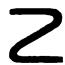
\includegraphics[keepaspectratio]{images/part002_d9406660.jpg}}

注意，若 \(\mathbf{A} \neq \mathbf{K}\) ，则一个 \(\neq \{0\}\) 的主分式理想不是把 \(\mathbf{K}\) 看作环时的理想。

主分式理想 Ax 也记作 \((x)\) 。我们将写 \(x \equiv 0 \pmod{y}\) 以表示 \(x \in Ay\) ，写 \(x \equiv x' \pmod{y}\) 以表示 \(x - x' \in Ay\) ；若 \(x \equiv x' \pmod{y}\) ，则 \(zx \equiv zx' \pmod{zy}\) 对任意 \(z \in K\) 成立。

注意，\(x \equiv x' (\bmod y)\) 并不蕴含 \(zx \equiv zx' (\bmod y)\) ，除非 \(z \in A\) 。因此在 \(\mathbf{Q}\) 中相对于 \(\mathbf{Z}\) ，有 \(4 \equiv 2 (\bmod 2)\) 但没有 \(2 \equiv 1 (\bmod 2)\) 。

关系 \(x \mid y\) 显然等价于 \((x) \supset (y)\) 。映射 \(x \mapsto (x)\) 从 \(K^*\) 映到集合 \(\mathcal{P}^*\) （由 \(\neq (0)\) 的、\(K\) 的主分式理想组成）上，从而在取商后定义了一个从 \(K^*/A^*\) 到 \(\mathcal{P}^*\) 的双射；借助这个映射把 \(K^*/A^*\) 的群结构转移到 \(\mathcal{P}^*\) 上，我们便被引导去把两个主分式理想 \((x)\) 与 \((y)\) 的乘积定义为理想 \((xy)\) ，它只依赖于 \((x)\) 与 \((y)\) 。配备了这个运算和序关系 \((x) \supset (y)\) 之后，集合 \(\mathcal{P}^*\) 构成一个序群，同构于 \(K^*/A^*\) 。按惯例，我们将通过上述映射把 \(\mathcal{P}^*\) 与 \(K^*/A^*\) 等同起来。

注意，在正整数情形下，“x 整除 y”这一关系意味着 x 小于 y，它对应于包含关系 \((x) \supset (y)\) ，其中理想 \((x)\) “大于”理想 \((y)\) 。我们可以记住这种“序反转”，例如注意到 7 的“倍数”比 91 的“更多”。

若我们把关系 \(x \mid y\) 扩展到 \(\mathbf{K}\) 的所有元素上，则此关系仍等价于 \((x) \supset (y)\) ，这里集合 \(\mathcal{P}\) 由 \(\mathbf{K}\) 的所有主分式理想组成（其中 (0) 在包含关系下是最小元素）。

如前几节一样，下文我们一般将使用加法记号。然而，与整除性有关的术语将跟在相应的加法术语之后引入，置于以记号（DIV）开头的段落中（其中约定使用本节的记号）。为方便读者，某些结果将被翻译成整除性的语言，例如命题7的翻译记作“命题7（DIV）”。

\subsection{序群的初等运算}

设H是序群G的一个子群；显然，G的序在H上的限制与H的群结构相容；除非另有说明，我们总按这种方式给H赋序。若P是G的正元素集合，则H的正元素集合是 \(H \cap P\) 。

设 \((\mathbf{G}_{\alpha})\) 是一族序群；根据有序集乘积的定义（集合论，III，第137页），乘积群 \(\mathbf{G} = \prod_{\alpha}\mathbf{G}_{\alpha}\) 装备着

一个序关系，G 的两个元素之间的关系 \(\ll (x_{\alpha}) \leqslant (y_{\alpha})\) 按定义等同于“ \(\ll x_{\alpha} \leqslant y_{\alpha}\) 对所有 \(\alpha\) ”。显然，这个序关系与G的群结构相容；它使G成为一个序群，我们称之为序群 \(G_{\alpha}\) 的乘积。G的正元素是那些所有分量均为正的元素。当所有因子 \(G_{\alpha}\) 都等于同一个序群H时，G就是由指标集I到H的映射组成的群 \(H^{I}\) ，从I到H的两个映射之间的关系 \(\ll f \leqslant g\) 就是“ \(\ll f(\alpha) \leqslant g(\alpha)\) 对所有 \(\alpha \in I\) ”；正映射是指只取正值的映射。序群族 \((G_{\alpha})\) 的直和定义为其乘积的一个序子群（II，第202页）。

设 \((\mathbf{G}_{\iota})_{\iota \in I}\) 是一族序群，其指标集 I 是良序的；回忆（集合论，III，第157页），在乘积集 \(\mathbf{G} = \prod_{\iota} \mathbf{G}_{\iota}\) 上定义了一个称为字典序的序关系，关系 \(\ll (x_{\iota}) < (y_{\iota})\)

（G 的两个元素之间）按定义等同于“若 β 是使得 \(x_{i} \neq y_{i}\) 的指标 i 中最小者，则 \(x_{\beta} < y_{\beta}\) ”。回忆，全序集的良序族的乘积在字典序下仍是全序的。在一般情形下，直接验证可知G上的字典序与其群结构相容；装备此序后，群G因此是一个序群，称为良序序群族的字典序积（ \(G_{i}\) ）。

注记. --- 1) 在最常见的情形中，良序指标集 I 将是一个有限区间 \([1, n]\) （包含在 \(\mathbf{N}\) 中）。

\begin{enumerate}
\def\labelenumi{\arabic{enumi})}
\setcounter{enumi}{1}
\tightlist
\item
  字典序乘积G的正元素集合由0以及那些非零元素组成，这些非零元素的最小索引非零分量为正。
\end{enumerate}

\subsection{序群的增同态}

设 G 和 \(G'\) 是两个序群；在从G的底层加法群到 \(G'\) 的底层加法群的同态中，考虑增映射是有意义的，即满足 \(x \leqslant y\) 蕴含 \(f(x) \leqslant f(y)\) 的那些映射。由于关系 \(f(y - x) = f(y) - f(x)\) ，由此可知，从 G 到 \(G'\) 的增同态的特征在于：在这样的同态下，G 的正元素的像是 \(G'\) 的正元素；若 P（相应地， \(P'\) ）表示 G（相应地，G'）的正元素集合，这可以写成 \(f(P) \subset P'\) 。显然，子群 G 到序群 G' 的典范单射，以及序群的乘积到其一个因子上的投影，都是增同态。

从序群 G 到序群 \(G'\) 上的一个同构（VI，第2页）f 是从 G 到 \(G'\) 上的双射同态，使得 f 与其逆同态都是增的，换言之， \(f(P) = P'\) 。

可能发生这样的情况：从 G 的底层群到 \(G'\) 的底层群的同构是增的，而逆同构却不是增的。例如，当 \(G = G'\) 时，若 f 是 G 上的恒等映射，且 \(P \subset P'\) 但 \(P \neq P'\) ，就是这种情形。因此在 Z 中，我们可以取 \(P'\) 为（通常意义的）正整数集合，而 P 为正偶整数集合。

(DIV) 设 K 是有理函数域 \(\mathbf{F}_{2}(\mathbf{X})\) （在 2 阶域 \(F_{2}\) 上）。相对于环 \(F_{2}[X] = A'\) 与环 \(F_{2}[X^{2}, X^{3}] = A\) 的整除关系在 \(K^{*}\) 上定义了两个不同的序群结构，它们满足 \(A \subset A'\) （它们确实是序群结构，因为 1 是 A 中唯一的单位，也是 \(A'\) 中唯一的单位）。

\subsection{序群中的上确界与下确界}

回忆（集合论，III，第141页），若子集 \(F\) （属于有序集 \(E\) ）的上界集合（也就是说，由这样的 \(z \in E\) 组成的集合： \(x \leqslant z\) 对所有 \(x \in F\) 成立）有一个最小元素 \(a\) ，则这个元素（届时是唯一的）称为 \(F\) 的上确界。若 \(F\) 是某个元素族 \((x_{i})_{i \in I}\) （其元素属于 \(E\) ）中元素的集合，则其上确界（若存在）记为 \(\sup_{i \in I} x_i\) （或记为 \(\sup_{i} x_i\) ，或简记为 \(\sup(x_i)\) ）；如果它是一个

有限族 \((x_{\iota})\) \((1 \leqslant \iota \leqslant n)\) ，则该上确界也记为 sup \((x_{1}, \ldots, x_{n})\) 。下确界的定义类似，记为 inf。运算 sup 和 inf 满足结合律和交换律。

回顾（集合论，同上引）若 F 是有序集 E 的一个子集，且 \((x_{t})\) 是 F 中元素的一个族，则 \(\sup(x_{t})\) 在 E 中的存在性（可记为 \(\sup_{E}(x_{t})\) ）并不蕴含 \(x_{t}\) 在 F 中的上确界的存在性（当它存在时可记为 \(\sup_{F}(x_{t})\) ）；若两者都存在，我们只知道 \(\sup_{E}(x_{t}) \leqslant \sup_{F}(x_{t})\) ；然而若 \(\sup_{E}(x_{t})\) 存在且属于 F，则 \(\sup_{F}(x_{t})\) 存在且等于 \(\sup_{E}(x_{t})\) 。例如，在多项式环 A = K{[}X, Y{]} （K 为域）中，主理想 AX 和 AY 在 A 的理想的有序集（按包含关系 ⊂）中具有上确界 AX + AY，但在 A 的所有主理想的集合中具有上确界 A。

（DIV）一个元素 \(d\) （属于 \(\mathbf{K}^*\) ）称为元素族 \((x_{\iota})\) （其元素属于 \(\mathbf{K}^*\) ）的最大公因子，简称 gcd，如果主分式理想 \((d)\) 是 \(\mathcal{P}^*\) 中（在关系 \(\subset\) 下）理想族 \(((x_{\iota}))\) 的上确界，或者换句话说，如果关系 \(z \mid d\) （ \(z \in \mathbf{K}^*\) ）等价于“ \(\ll z \mid x_{\iota}\) 对所有 \(\iota\) ”。同样地，我们将说 \(m \in \mathbf{K}^*\) 是族 \((x_{\iota})\) 的最小公倍元或 lcm，如果 \((m)\) 是 \(\mathcal{P}^*\) 中理想族 \(((x_{\iota}))\) 的下确界，即 \(m \mid z\) 等价于“ \(\ll x_{\iota} \mid z\) 对所有 \(\iota\) ”。这等同于说 \((m) = \bigcap_{\iota} (x_{\iota})\) ；事实上，条件 \(x_{\iota} \mid z\) （对所有 \(\iota\) ）等价于 \(z \in Ax_{\iota}\) （对所有
\(\iota\) ），即 \(z \in \cap (x_{\iota})\) ，而条件 \(m \mid z\) 等价于 \(z \in (m)\) \(^{1}\) 。

\pandocbounded{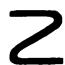
\includegraphics[keepaspectratio]{images/part002_2ca33fff.jpg}}

注意，若主分式理想 \((d)\) 满足 \((d) = \sum_{i} (x_i)\) ，则 \(d\) 是族 \((x_{\iota})\) 的一个最大公因子；但反过来， \((x_{\iota})\) 的最大公因子不一定满足上述条件（参见第六章，第33页，习题24）。

最大公因子和最小公倍元若存在，则在 \(K^{*}\) 的单位组成的子群 U 的模下是良定义的，也就是说，给定族的两个最大公因子（或两个最小公倍元）是相伴元；按语言的滥用，我们常把 \(\gcd(x_{t})\) 与 \(\operatorname{lcm}(x_{t})\) 写作族 \((x_{t})\) 的任意一个最大公因子或最小公倍元，只要这样的元素存在。

（DIV）按语言的滥用，我们有时把最大公因子的概念推广到 K 的元素的族 \((x_{i})\) ，其中某些元素可以是零；这个最大公因子仍定义为这样的元素 d：关系 \(z \mid d\) 等价于“ \(z \mid x_{i}\) 对所有 \(i\) ”；显然，若所有 \(x_{i}\) 均为零，则 d 为零；否则 d 是非零 \(x_{i}\) 的最大公因子。类似地，若一族元素中有一些为零，则其最小公倍元为 0。

在序群 G 中，序在平移下的不变性（VI，第 2 页，命题 2）的一个直接推论是

\[
\sup \left(z + x _ {i}\right) = z + \sup \left(x _ {i}\right)\tag{1}
\]

其含义是，只要一边有定义，则另一边也有定义且两者相等。类似地，由映射 \(x \mapsto -x\) 将 G 的序变为相反序（VI，第 3 页，推论）这一事实可得

\[
\inf (- x _ {i}) = - (\sup (x _ {i})),\tag{2}
\]

此关系与前一个关系作相同理解。

命题6. --- 设 \((x_{\alpha})_{\alpha \in A}, (y_{\beta})_{\beta \in B}\) 是序群G中元素的两个族，每个族都有上确界。则族 \((x_{\alpha} + y_{\beta})_{(\alpha, \beta) \in A \times B}\) 具有上确界，并且 \(\sup_{(\alpha, \beta) \in A \times B} (x_{\alpha} + y_{\beta}) = \sup_{\alpha \in A} x_{\alpha} + \sup_{\beta \in B} y_{\beta}\) 。

确实，由 \(x_{\alpha} + y_{\beta} \leqslant z\) （对所有 \(\alpha\) 与 \(\beta\) ）可推出 \(\sup (x_{\alpha}) + y_{\beta} \leqslant z\) （对所有 \(\beta\) ），从而 \(\sup (x_{\alpha}) + \sup (y_{\beta}) \leqslant z\) 。

\subsection{格序群}

回忆，其中每个非空有限子集都有上确界和下确界的有序集称为格（E，III，第13页）。显然，格序群的乘积，特别地全序群的乘积，是格序群。与此相反，格序群的子群不一定是格序的。

于是，在乘积序群 \(\mathbf{Z} \times \mathbf{Z}\) 中，“反对角线”（数对 \((n, n')\) ——满足 \(n + n' = 0\) ——组成的集合）装备离散序，因此不是格序群。* 单个实变量的多项式加法群（VI，第1页，例2）是滤过群（因为 \(p(x)\) 与 \(q(x)\) 都小于 \((p(x))^2 + (q(x))^2 + 1\) ），可以证明它不是格序的。*

命题7. --- 若 \(x\) 与 \(y\) 是序群 \(G\) 的两个元素，且元素 \(\inf(x, y)\) , \(\sup(x, y)\) 之一存在，则另一个也存在，并且 \(x + y = \inf(x, y) + \sup(x, y)\) 。

事实上，根据关系式(1)和(2)（VI，第9页），我们有

\[
\sup (a - x, a - y) = a + \sup (- x, - y) = a - \inf (x, y),
\]

只需取 \(a = x + y\) 即可。

命题7（DIV）。 --- 若 \(a, b \in \mathbf{K}^{*}\) ，且若 \(d\) 是 \(a\) 与 \(b\) 的一个最大公因子，而 \(m\) 是 \(a\) 与 \(b\) 的一个最小公倍元，则乘积 dm 是 \(ab\) 的相伴元。

命题 8. --- 设P是序群G的正元素集合。要使G是格序群，必要且充分的是G = P - P，且此外P（装备诱导序）满足下列两个条件之一：

\begin{enumerate}
\def\labelenumi{\alph{enumi})}
\item
  \(\mathbf{P}\) 的每一对元素在 \(\mathbf{P}\) 中都有上确界。
\item
  \(\mathbf{P}\) 的每一对元素在 \(\mathbf{P}\) 中都有下确界。
\end{enumerate}

这些条件的必要性是显然的：事实上，关系 \(G = P - P\) 表明G是滤过的（VI，第4页，命题4）；另一方面，P的两个元素在G中的上确界和下确界是正的，因而它们也是这两个元素在P中的上确界和下确界。

反过来，首先注意到在假设a)（相应地，b)）下，P中任意一对元素x、y在G中的上确界（相应地，下确界）等于其在P中的上确界a（相应地，下确界b）。这对a)是显然的，因为x和y的任何上界都是正的；对于b)，设 \(z \in G\) 是 x 和 y 的一个下界；则存在 \(u \in P\) 使得 \(z + u \in P\) ，因为 G = P - P；现在 \(\inf_{P}(x + u, y + u)\) 大于或等于 \(b + u\) ，因此具有形式 \(b + c + u\) ( \(c \geqslant 0\) ）；因为 \(b + c\) 小于x且小于y，我们有 c = 0；因此 \(\inf_{P}(x + u, y + u) = b + u\) ，这意味着 \(z + u \leqslant b + u\) ，因此 \(z \leqslant b\) 且 b 显然是 x 和 y 在 G 中的下确界。现在若 x 和 y 是 G 的任意元素，我们将它们平移进 P：令 \(v \in P\) 使得 \(x + v\) 与 \(y + v\) 都是正的（VI，第 5 页，命题 5）；在假设 a)（相应地 b)）下

\(x + v\) 与 \(y + v\) 在 P 中存在上确界（相应地，下确界），因而根据刚才所证，在 G 中也存在；通过平移，x 和 y 在 G 中有上确界（相应地，下确界）；由命题7，其中一个的存在蕴含另一个的存在，这就表明这些条件是充分的。

\subsection{分解定理}

定理1（分解定理）. --- 设 \((x_i)_{1 \leq i \leq p}\) 与 \((y_j)_{1 \leq j \leq q}\) 是格序群 \(G\) 中正元素的两个有限序列，满足 \(\sum_{i=1}^{p} x_i = \sum_{j=1}^{q} y_j\) ；则存在正元素的一个双重序列 \((z_{ij})_{1 \leq i \leq p, 1 \leq j \leq q}\) （属于 \(G\) ），使得 \(x_i = \sum_{j=1}^{q} z_{ij}\) （对所有 \(i\) ），并且 \(y_j = \sum_{i=1}^{p} z_{ij}\) （对所有 \(j\) ）。

\begin{enumerate}
\def\labelenumi{\arabic{enumi})}
\tightlist
\item
  我们首先对 \(p = q = 2\) 的情形证明该定理。设 \(x, x', y, y'\) 是 \(G\) 的正元素，满足 \(x + x' = y + y'\) ，并令 \(a = \sup (0, x - y')\) 。由于
\end{enumerate}

\[
x - y ^ {\prime} = y - x ^ {\prime}
\]

小于 \(x\) 且小于 \(y\) ，由此可得 \(b = x - a\) 与 \(c = y - a\) 是正的， \(d = a - (x - y')\) 也是正的。此外我们还有

\[
x = a + b, x ^ {\prime} = c + d, y = a + c \quad \text { and } \quad y ^ {\prime} = b + d.
\]

\begin{enumerate}
\def\labelenumi{\arabic{enumi})}
\setcounter{enumi}{1}
\tightlist
\item
  现在我们证明：若定理对 \(p < m\) 与 \(q = n\) ( \(m > 2\) , \(n \geqslant 2\) )成立，则它对 \(p = m\) 与 \(q = n\) 也成立。根据假设，我们有 \(x_{m} + \sum_{i=1}^{m-1} x_{i} = \sum_{j=1}^{n} y_{j}\) 。由于定理对 \(p = 2\) 与 \(q = n\) 成立，故存在两个有限序列 \((z_{j}')\) , \((z_{j}''')\) （各由 \(n\) 个正项组成），使得 \(\sum_{i=1}^{m-1} x_{i} = \sum_{j=1}^{n} z_{j}'\) , \(x_{m} = \sum_{j=1}^{n} z_{j}''\) ，并且 \(y_{j} = z_{j}' + z_{j}''\) （对 \(1 \leqslant j \leqslant n\) ）。另一方面，由于定理对 \(p = m-1\) 与 \(q = n\) 成立，存在一个双重序列 \((u_{ij})_{1 \leqslant i \leqslant m-1, 1 \leqslant j \leqslant n}\) ，使得 \(x_{i} = \sum_{j=1}^{n} u_{ij}\) （对 \(1 \leqslant i \leqslant m-1\) ），并且 \(z_{j}' = \sum_{i=1}^{m-1} u_{ij}\) （对 \(1 \leqslant j \leqslant n\) ）。令
\end{enumerate}

\[
z _ {i j} = u _ {i j} \quad \text { for } \quad 1 \leqslant i \leqslant m - 1, \quad \text { and } \quad z _ {m j} = z _ {j} ^ {\prime \prime} \quad (1 \leqslant j \leqslant n),
\]

我们便确实得到一个满足定理条件的双重序列。3) 通过交换 \(x_{i}\) 与 \(y_{j}\) ，我们以同样的方式看到，若定理对 \(p = m\) 与 \(q < n\) ( \(m \geqslant 2\) , \(n > 2\) )成立，则它对 \(p = m\) 与 \(q = n\) 也成立。于是定理通过从 \(p = q = 2\) 情形出发的双重归纳法得到证明，因为只要 \(p \leqslant 1\) 或 \(q \leqslant 1\) ，它是平凡成立的。

推论。 --- 设 \(y, x_1, x_2, \ldots, x_n\) 是 \(n + 1\) 个正元素（属于 \(G\) ），满足 \(y \leqslant \sum_{i=1}^{n} x_i\) ；则存在 \(n\) 个正元素 \(y_i (1 \leqslant i \leqslant n)\) ，使得 \(y_i \leqslant x_i\) 且 \(y = \sum_{i=1}^{n} y_i\) 。

只需对序列 \((x_{i})\) 以及由两个元素 \(y\) 与 \(z = \left(\sum_{i=1}^{n} x_{i}\right) - y\) 组成的序列应用定理1。

\subsection{正部与负部}

定义4. --- 在格序群G中，元素 \(x \in G\) 的正部（相应地，负部，绝对值）是元素 \(\sup(x, 0)\) （相应地 \(\sup(-x, 0)\) , \(\sup(x, -x)\) ），记作 \(x^{+}\) （相应地 \(x^{-}\) , \(|x|\) ）。

\pandocbounded{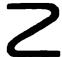
\includegraphics[keepaspectratio]{images/part002_7ee71349.jpg}}

尽管名称如此，负部 \(x^{-}\) 是一个正元素。

显然 \(x^{-} = (-x)^{+}\) 且 \(|-x| = |x|\) 。我们还注意到下列公式，其中第一个是定义以及序在平移下的不变性的直接推论，第二个则由第一个根据VI第10页命题7得出：

\[
\left\{ \begin{array}{l} \sup (x, y) = x + (y - x) ^ {+}, \\ \inf (x, y) = y - (y - x) ^ {+}. \end{array} \right.\tag{3}
\]

命题9. --- a) 对格序群G的每个元素 x，我们有 \(x = x^{+} - x^{-}\) 且 \(\inf(x^{+}, x^{-}) = 0\) 。

\begin{enumerate}
\def\labelenumi{\alph{enumi})}
\setcounter{enumi}{1}
\item
  对 \(x\) 作为两个正元素之差的每一种表示，设 \(x = u - v\) ，我们有 \(u = x^{+} + w\) 与 \(v = x^{-} + w\) ，其中 \(w = \inf(u, v)\) 。特别地，若 \(\inf(u, v) = 0\) ，则 \(u = x^{+}\) 且 \(v = x^{-}\) 。
\item
  关系 \(\ll x\leqslant y\gg\) 等价于 \(\ll x^{+}\leqslant y^{+}\) 且 \(x^{-}\geqslant y^{-}\gg\) 。
\item
  我们有 \(|x| = x^{+} + x^{-} \geqslant 0\) 。
\item
  对任意 \(x\) 与 \(y\) （在 \(G\) 中），我们有不等式 \(|x + y| \leqslant |x| + |y|\) ，并且更一般地 \(\left|\sum_{i=1}^{n} x_i\right| \leqslant \sum_{i=1}^{n} |x_i|\) （对元素的任意有限族 \((x_i)\) ，其元素属于 \(G\) ）。
\item
  对任意 \(x\) 与 \(y\) （在 \(G\) 中），我们有 \(||x| - |y|| \leqslant |x - y|\) 。
\end{enumerate}

我们将同时证明 \(a)\) 与 \(b)\) 。若 \(x = u - v\) ，其中 \(u\) 与 \(v\) 为正，则 \(u \geqslant x\) ，所以 \(u \geqslant \sup (x, 0) = x^{+}\) ，且 \(w = u - x^{+}\) 为正。另一方面，我们有

\[
x ^ {+} - x = \sup (x, 0) - x = \sup (x - x, - x) = x ^ {-}
\]

由此可得 \(x = x^{+} - x^{-}\) ，以及 \(v - x^{-} = w\) 。若 \(z \leqslant x^{-}\) ，则 \(z \leqslant x^{+} - x\) ，因此 \(x \leqslant x^{+} - z\) ；若还有 \(z \leqslant x^{+}\) ，则 \(x^{+} - z\) 是正的，因此 \(x^{+} \leqslant x^{+} - z\) （按 \(x^{+}\) 的定义）。于是我们有 \(z \leqslant 0\) ，这意味着 \(\inf(x^{+}, x^{-}) = 0\) ，从而通过平移得到 \(\inf(u, v) = w\) 。

\begin{enumerate}
\def\labelenumi{\alph{enumi})}
\setcounter{enumi}{2}
\item
  关系 \(x \leqslant y\) 蕴含 \(\sup (y, 0) \geqslant x\) 与 \(\sup (y, 0) \geqslant 0\) ，因此 \(x^{+} \leqslant y^{+}\) ；类似地，若 \(-y \leqslant -x\) ，我们推出 \(x^{-} \geqslant y^{-}\) 。相反的蕴含关系由 \(x = x^{+} - x^{-}\) 与 \(y = y^{+} - y^{-}\) 立即得出。
\item
  由于 \(x \leqslant x^{+}\) 且 \(-x \leqslant x^{-}\) ，显然
\end{enumerate}

\[
\left| x \right| = \sup (x, - x) \leqslant x ^ {+} + x ^ {-}.
\]

反之，若 \(a \geqslant x\) 且 \(a \geqslant -x\) ，则由 \(c\) ) 推出 \(a^+ \geqslant x^+\) , \(a^+ \geqslant x^-\) , \(a^- \leqslant x^-\) 与 \(a^- \leqslant x^+\) ；由于 \(a^-\) 是正的且 \(\inf(x^+, x^-) = 0\) ，后两个不等式推出 \(a^- = 0\) 且 \(a = a^+\) ；前两个不等式随后给出 \(a \geqslant \sup(x^+, x^-)\) ，而 \(\sup(x^+, x^-)\) 等于 \(x^+ + x^-\) （由 \(a\) ）以及VI第10页命题7）。

\begin{enumerate}
\def\labelenumi{\alph{enumi})}
\setcounter{enumi}{4}
\item
  由于 \(x \leqslant |x|\) 且 \(y \leqslant |y|\) ，我们有 \(x + y \leqslant |x| + |y|\) ；由于 \(-x \leqslant |x|\) 且 \(-y \leqslant |y|\) ，我们有 \(-x - y \leqslant |x| + |y|\) ；由此得到第一个不等式。第二个不等式通过对 \(n\) 作归纳得到。
\item
  把 \(x\) 与 \(y\) 分别换成 \(y\) 与 \(x - y\) （在 \(e\) ) 中），我们得到
\end{enumerate}

\[
\left| x \right| - \left| y \right| \leqslant \left| x - y \right|;
\]

类似地，我们有 \(|y| - |x| \leqslant |y - x| = |x - y|\) ；由此得出所述结果。

注记. --- 我们由 \(d\) 推出， \(|x|=0\) 蕴含 \(x=0\) （因为 \(x^{+}\) 与 \(x^{-}\) 都是正的）；于是 \(x\neq0\) 蕴含 \(|x|>0\) 。

命题9（DIV）. --- 若由 K 的主分式理想组成的群 \(\mathcal{P}^*\) 是格序的，则每个元素 \(x\) （属于 \(\mathbf{K}^*\) ）都可以写成 \(x = uv^{-1}\) 的形式，其中 \(u\) 与 \(v\) 是 A 的元素，满足 \(1 = \gcd(u, v)\) ；对任何其他表达式 \(x = u'v'^{-1}\) （它把 \(x\) 表示为 A 中两个元素之商） ，我们有 \(u' = uw\) 与 \(v' = vw\) ，其中 \(w\) 是 \(u'\) , \(v'\) 的一个最大公因子；特别地，若 \(1 = \gcd(u', v')\) ，则 \(u'\) 与 \(v'\) 分别是 \(u\) 与 \(v\) 的相伴元。

这样一个表达式 \(uv^{-1}\) （对 \(K^{*}\) 中一个元素 x 而言）通常称为既约分数。

\subsection{互素元}

定义 5. --- 在序群中，两个元素 x 与 y 称为互素的，如果 \(\inf(x, y) = 0\) 。

在某些情形下，把满足 \(\inf(|x|, |y|) = 0\) 的两个元素定义为互素是自然的（参见 INT，II，§ 1），或者在整除理论中引入相应的术语。我们不这样做。

两个互素元素必定是正的。x 的正部和负部 \(x^{+}\) 与 \(x^{-}\) 是互素的（VI，第12页，命题9 a））。元素 \(x_{i}\) （属于某个族 \((x_{t})_{t\in I}\) ）称为整体互素的，如果 \(\inf_{t\in I}x_t = 0\) ；若这些 \(x_{t}\) 都 \(\geqslant 0\) ，则

只需存在 I 的一个有限子集 J，使得相应的元素整体互素。族 \((x_{\iota})\) 的元素称为两两互素的，如果 \(\inf(x_{\iota}, x_{\kappa}) = 0\) 对每对不同的指标 \((\iota, \kappa)\) 成立。

诸 \(x_{i}\) 可以整体互素而不两两互素。

若 \(x\) 与 \(y\) 是互素的，我们也说 \(x\) 与 \(y\) 互素，或说 \(y\) 与 \(x\) 互素。

（DIV）K 的两个元素 x 与 y 称为互素的，如果主理想 \((x)\) 与 \((y)\) 在 \(P^{*}\) 中非零且互素；这等于说 1 是 x 与 y 的一个最大公因子，并蕴含 x 与 y 属于 A。例如，既约分数的分子与分母是互素的。两两互素元素和整体互素元素的概念可类似地定义。

（DIV）当 \(x\) 与 \(y\) 互素时，常称它们“彼此互素”；宜避免这一术语，它可能与素数的概念（I，第50页，定义16）混淆。

命题 10. --- 设 \(x, y\) 与 \(z\) 是序群的三个元素；要使 \(x - z\) 与 \(y - z\) 互素，必要且充分的是 \(z = \inf(x, y)\) 。

事实上，关系 \(z = \inf (x, y)\) 与 \(0 = \inf (x - z, y - z)\) 是等价的。

命题10（DIV）。 --- 设 \(a, b\) 与 \(c\) 是 \(\mathbf{K}\) 的三个元素，且 \(c \neq 0\) ；要使商 \(ac^{-1}\) 与 \(bc^{-1}\) 互素，必要且充分的是 \(c\) 是 \(a\) 与 \(b\) 的一个最大公因子。

命题11. --- 若 \((x_{i})\) , \((y_{j})\) 是格序群中正元素的两个有限族，则

\[
\inf \left(\sum_ {i} x _ {i}, \sum_ {j} y _ {j}\right) \leqslant \sum_ {i, j} \inf (x _ {i}, y _ {j}).
\]

对族 \((x_{i})\) 与 \((y_{j})\) 的元素个数进行归纳论证，只需证明：如果 \(x, y\) 与 \(z\) 是正元素，则

\[
\inf (x, y + z) \leqslant \inf (x, y) + \inf (x, z).
\]

事实上，令 \(t = \inf(x, y + z)\) ；由VI第12页的推论，我们可以写 \(t = t_1 + t_2\) ，其中 \(0 \leqslant t_1 \leqslant y\) 且 \(0 \leqslant t_2 \leqslant z\) ；由于 \(t_1\) 与 \(t_2\) 为正，我们还有 \(t_1 \leqslant x\) 与 \(t_2 \leqslant x\) ，从而 \(t_1 \leqslant \inf(x, y)\) 与 \(t_2 \leqslant \inf(x, z)\) 。

推论1. --- 若x与y是格序群的两个互素元，且z是一个正元素，则 \(\inf(x, z) = \inf(x, y + z)\) 。

事实上， \(\inf (x,y + z)\leqslant \inf (x,z)\) 由命题11得出，且 \(\inf (x,z)\leqslant \inf (x,y + z)\) 由 \(y\geqslant 0\) 得出，由此即得推论。

推论2. --- 在格序群中，若x与y互素，且 \(z \geqslant 0\) 与 \(x \leqslant y + z\) ，则 \(x \leqslant z\) 。

推论3. --- 在一个格序群中，如果x与y互素且与z互素，则x也与 \(y + z\) 互素。

推论4. --- 如果 \((x_i)_{1 \leq i \leq n}\) 与 \((y_j)_{1 \leq j \leq m}\) 是格序群G中元素的两个有限族，使得每个 \(x_i\) 与每个 \(y_j\) 互素，则 \(x_1 + \cdots + x_n\) 与 \(y_1 + \cdots + y_m\) 互素。

这由推论3通过对m和n进行归纳得出。

推论5. --- 对任意整数 \(n \geqslant 0\) ，我们有 \((nx)^+ = nx^+\) 与 \((nx)^- = nx^-\) ；对所有 \(n \in \mathbf{Z}\) ，我们有 \(|nx| = |n| \cdot |x|\) 。

事实上， \(nx = nx^{+} - nx^{-}\) ；由于 \(x^{+}\) 与 \(x^{-}\) 互素，因此 \(nx^{+}\) 与 \(nx^{-}\) 在 \(n \geqslant 0\) 时也互素（推论4）；第一个断言由VI第12页命题9 b)得出。第二个断言在情形 \(n \geqslant 0\) 下由第一个断言根据命题9 d)得出；情形 \(n < 0\) 由此根据关系 \(|-x| = |x|\) 得出。

命题11（DIV）。--- 假设集合 \(\mathcal{P}^*\) 是一个格，并设 \((a_i)\) , \((b_j)\) 为A中元素的两个有限族。则 \(\prod_{i} a_i\) 与

\(\prod_{j} b_{j}\) 的每一个最大公因子都整除乘积 \(\prod_{i,j} \gcd(a_{i}, b_{j})\) 。

推论1（DIV）。--- 若 a、b、c 是A的三个元素，且a与b互素，则a与c的每个最大公因子也是a与bc的一个最大公因子。

推论2（DIV）（欧几里得引理）。--- 设 \(a, b, c\) 是A的三个元素。如果 \(a\) 与 \(b\) 互素且整除 \(bc\) ，则它整除 \(c\) 。

推论3（DIV）。--- 若x与y互素且与z互素，则x与yz互素。

推论4（DIV）。--- 如果 \((x_{i})\) 与 \((y_{j})\) 是A中元素的两个有限族，使得每个 \(x_{i}\) 与每个 \(y_{j}\) 互素，则这些 \(x_{i}\) 的乘积与这些 \(y_{j}\) 的乘积互素。

推论5（DIV）。--- 如果 \(d\) 是 \(x\) 与 \(y\) 的一个最大公因子，则 \(d^n\) 是 \(x^n\) 与 \(y^n\) 的一个最大公因子（对每个正整数 \(n\) ）。

事实上， \(xd^{-1}\) 与 \(yd^{-1}\) 互素（命题10（DIV）），因此 \(x^{n}d^{-n}\) 与 \(y^{n}d^{-n}\) 也互素（推论4）。

命题12. --- 设 \(x_{i}\) ( \(1 \leqslant i \leqslant n\) ) 是格序群中 \(n\) 个两两互素的元素。则

\[
\sup \left(x _ {1}, \dots , x _ {n}\right) = x _ {1} + \dots + x _ {n}.
\]

这由公式 \(u + v = \sup(u, v) + \inf(u, v)\) （VI，第10页，命题7）通过对n归纳得出，其中用到 \(x_{i}\) 与 \(x_{1} + \cdots + x_{i-1}\) 互素这一事实， \(2 \leqslant i \leqslant n\) （命题11的推论4）。

注. --- VI第10页命题7还表明， \(x\) 与 \(y\) 互素的一个充分必要条件是 \(x + y = \sup(x, y)\) 。

命题12（DIV）。--- 设 \(a_i\) 是 \(n\) 个属于 \(A\) 的两两互素的元素；则乘积 \(a_1 \ldots a_n\) 是 \(a_1, \ldots, a_n\) 的一个最小公倍元。

命题13. --- 在格序群G中，设 \((x_{\alpha})\) 是一个具有下确界（相应地，上确界）的族，并设 z 为 G 的任意元素；则族 \((\sup(z, x_{\alpha}))\) （相应地 \((\inf(z, x_{\alpha})))\) 具有下确界（相应地，上确界）且

\[
\left\{ \begin{array}{l} \inf _ {\alpha} (\sup (z, x _ {\alpha})) = \sup \left(z, \inf _ {\alpha} x _ {\alpha}\right) \\ \sup _ {\alpha} (\inf (z, x _ {\alpha})) = \inf \left(z, \sup _ {\alpha} x _ {\alpha}\right) \end{array} \right.\tag{4}
\]

（相应地）。

假设族 \((x_{\alpha})\) 具有下确界 \(y\) 。我们将证明 \(\sup (z,y)\) 是族 \((\sup (z,x_{\alpha}))\) 的一个下确界。

事实上， \(\sup (z, x_{\alpha}) = z + (x_{\alpha} - z)^{+}\) ，通过平移我们可以归结为 \(z = 0\) 的情形，即我们必须证明 \((x_{\alpha}^{+})\) 的下确界等于 \(y^{+}\) 。由于 \(y \leqslant x_{\alpha}\) ，我们有 \(y^{+} \leqslant x_{\alpha}^{+}\) 对所有 \(\alpha\) 成立（VI，第12页，命题9 c））。反之，若 \(a \leqslant x_{\alpha}^{+}\) 对所有 \(\alpha\) ，则由此可得 \(a \leqslant x_{\alpha} + x_{\alpha}^{-}\) （命题9 a））；现在 \(y^{-} \geqslant x_{\alpha}^{-}\) ，因为 \(y \leqslant x_{\alpha}\) ；因此 \(a \leqslant x_{\alpha} + y^{-}\) 对所有 \(\alpha\) ，即 \(a \leqslant y + y^{-} = y^{+}\) 。

另一公式通过改为相反的序关系即可得出。

推论. --- 若格序群G的元素z与某个下确界为y的族的每个元素 \(x_{\alpha}\) 互素，则z与y互素。

这是公式 (4) 中第二个公式的直接推论。

注. --- 将命题13的公式应用于由两个元素 \((x, y)\) 组成的族，我们得到以下公式，它们表达了格序群中的两个合成律 sup、inf 各自对另一个的分配性：

\[
\begin{array}{l} \sup (z, \inf (x, y)) = \inf (\sup (z, x), \sup (z, y)) \\ \inf (z, \sup (x, y)) = \sup (\inf (z, x), \inf (z, y)). \end{array}
\]

这一分配性质是格序群所特有的，并不推广到任意格，甚至不推广到格序幺半群（参见VI，第33页，习题24）。
